\documentclass{beamer}
 
 
 \usepackage[utf8]{inputenc}
 \usepackage[T1]{fontenc}
 \usepackage[french]{babel}
 \usepackage{mathtools, bm}
 \usepackage{amssymb, bm}
 \usepackage{stmaryrd} 
 \usepackage{enumitem}
 \usepackage{xcolor}
 \usepackage{array}
 \usepackage{layout}
 \usepackage{pslatex}
 \usepackage{pstricks-add}
 \usepackage{lmodern}
 \usepackage{listings}
 \usepackage{color}
 \usepackage{pstricks,pst-node,pst-tree}
 \usepackage{tikz}
 \usepackage{mathrsfs} 
 \usepackage{media9}

 % le thème artisanal :
 \usetheme{Warsaw}
 \usecolortheme{seahorse}
 \useoutertheme{infolines}
 \setbeamercolor{block body}{bg=normal text.bg!95!black!95!blue}
 \setbeamercolor{block body example}{bg=normal text.bg!95!black!95!green}
 \setbeamercolor{block title}{fg=white, bg=normal text.bg!50!blue!50!black}
 \setbeamercolor{block title example}{fg=white,bg=normal text.bg!50!green!50!black}
 \useinnertheme{rounded}
 \setbeamertemplate{blocks}[rounded][shadow=true]
 \beamertemplatenavigationsymbolsempty
 \renewcommand{\arraystretch}{1.5}


% blocs 
 \newcommand{\prop}[1]{\begin{block}{Proposition}#1\end{block}}
 \newcommand{\thm}[2]{\begin{block}{Théorème (#1)}#2\end{block}}
 \newcommand{\conj}[1]{\begin{exampleblock}{Conjecture}#1\end{exampleblock}}
 \newcommand{\defi}[1]{\begin{exampleblock}{Définition}#1\end{exampleblock}}
 \newcommand{\exmp}[1]{\begin{exampleblock}{Exemple}#1\end{exampleblock}}
 \newcommand{\diapo}[1]{\begin{frame}[allowframebreaks]#1\end{frame}}
 \newcommand{\dem}{\textbf{Démonstration }\hspace{0.5cm}}



 \newcommand{\Iff}[2]{\left[#1\,;\,#2\right]}
 \newcommand{\Ioo}[2]{\left]#1\,;\,#2\right[}
 \newcommand{\Ifo}[2]{\left[#1\,;\,#2\right[}
 \newcommand{\Iof}[2]{\left]#1\,;\,#2\right]}



 \newcommand{\pth}[1]{\left(#1\right)}
 \newcommand{\cro}[1]{\left[#1\right]}
 \newcommand{\acc}[1]{\left\{#1\right\}}
 \newcommand{\abs}[1]{\left|#1\right|}
 \newcommand{\dabs}[1]{\|#1\|}
 \newcommand{\scal}[1]{\left<#1\right>}
 \newcommand{\floor}[1]{\left\lfloor#1\right\rfloor}
 \newcommand{\ceil}[1]{\left\lceil#1\right\rceil}
 \newcommand{\dbcro}[1]{\left\llbracket#1\right\rrbracket}


 % pour faire des commentaires cool

 \newcommand{\esp}{\hspace{1cm}}
 \newcommand{\et}{\hspace{1cm}\text{et}\hspace{1cm}}
 \newcommand{\pet}{\hspace{0.5cm}\text{et}\hspace{0.5cm}}
 \newcommand{\ou}{\hspace{1cm}\text{ou}\hspace{1cm}}
 \newcommand{\pou}{\hspace{0.5cm}\text{ou}\hspace{0.5cm}}
 \newcommand{\avec}{\hspace{1cm}\text{avec}\hspace{1cm}}
 \newcommand{\comment}[1]{\hspace{1cm}\text{#1}\hspace{1cm}}
 \newcommand{\tq}{\hspace{0.25cm}/ \hspace{0.25cm}}
 \newcommand{\qt}[1]{(\,#1\,)\hspace{1cm}}
 \newcommand{\qti}[1]{\,,\hspace{1cm}#1}
 \newcommand{\vg}{,\,}

 \newcommand{\ssi}{\hspace{.2cm}\Leftrightarrow\hspace{.2cm}}
 \newcommand{\gssi}{\hspace{1cm}\Leftrightarrow\hspace{1cm}}


 % Pour la géométrie
 \newcommand{\vect}[1]{\overrightarrow{#1}}
 
 % divers 

 \newcommand{\mat}[1]{\begin{matrix} #1\end{matrix}}
 \newcommand{\pmat}[1]{\begin{pmatrix} #1\end{pmatrix}}
 \newcommand{\cotan}{\text{cotan}}
 \newcommand{\somme}[2]{\sum_{#1=0}^{#2}}
 \newcommand{\Vect}[1]{\text{vect}\pth{#1}}
 \newcommand{\ie}{\emph{ie} }
 \newcommand{\transp}{{}^t\!}
 \newcommand{\lleq}{<\!\!\!<}
 

 % pour les intégrales:
 \newcommand{\bigcro}[1]{\big[#1\big]}
 \newcommand{\de}{\,\text{d}}


 % Les ensembles:
 \newcommand{\Ce}{\mathbb{C}}
 \newcommand{\Er}{\mathbb{R}}
 \newcommand{\En}{\mathbb{N}}
 \newcommand{\Zed}{\mathbb{Z}}
 \newcommand{\Qu}{\mathbb{Q}}
 \newcommand{\Te}{\mathbb{T}}

 % En probas
 \newcommand{\prb}[1]{\mathbb{P}\pth{#1}}
\newcommand{\Esp}[1]{\mathbb{E}\cro{#1}}
 \newcommand{\Var}[1]{\text{Var}\pth{#1}}
\newcommand{\kt }{\,|\,}

\newcommand{\edistr }{\overset{d}{=}}
\newcommand{\cdistr }{\overset{d}{\to}}
\newcommand{\cproba}{\overset{\mathbb{P}}{\to}}
\newcommand{\easrly}{\overset{a.s.}{=}}
\newcommand{\casrly}{\overset{a.s.}{\to}}


 % spécifique

\newcommand{\dr}{\partial}
\newcommand{\fr}{\mathcal{F}}

 \title[Mutations]{Estimer les effets des mutations sur la valeur sélective d’une bactérie}
 \date[2020 -- 2021]{Encadrantes : Marie Doumic et Lydia Robert}
 \author[J. Andréoletti, N. Boutillon]{Jérémy Andréoletti et Nathanaël Boutillon}

\begin{document}


\begin{frame}
  \titlepage
\end{frame}


\begin{frame}
  \frametitle{Objectifs}
  \begin{itemize}[label=$\bullet$]
  \item Comprendre la dynamique d'apparition des mutations, chez \emph{E. coli}
  \item Estimer la \textbf{DFE = Distribution des Effets des mutations sur la Fitness}
  \end{itemize}
  
  \vspace{3mm}

  \begin{centering}
    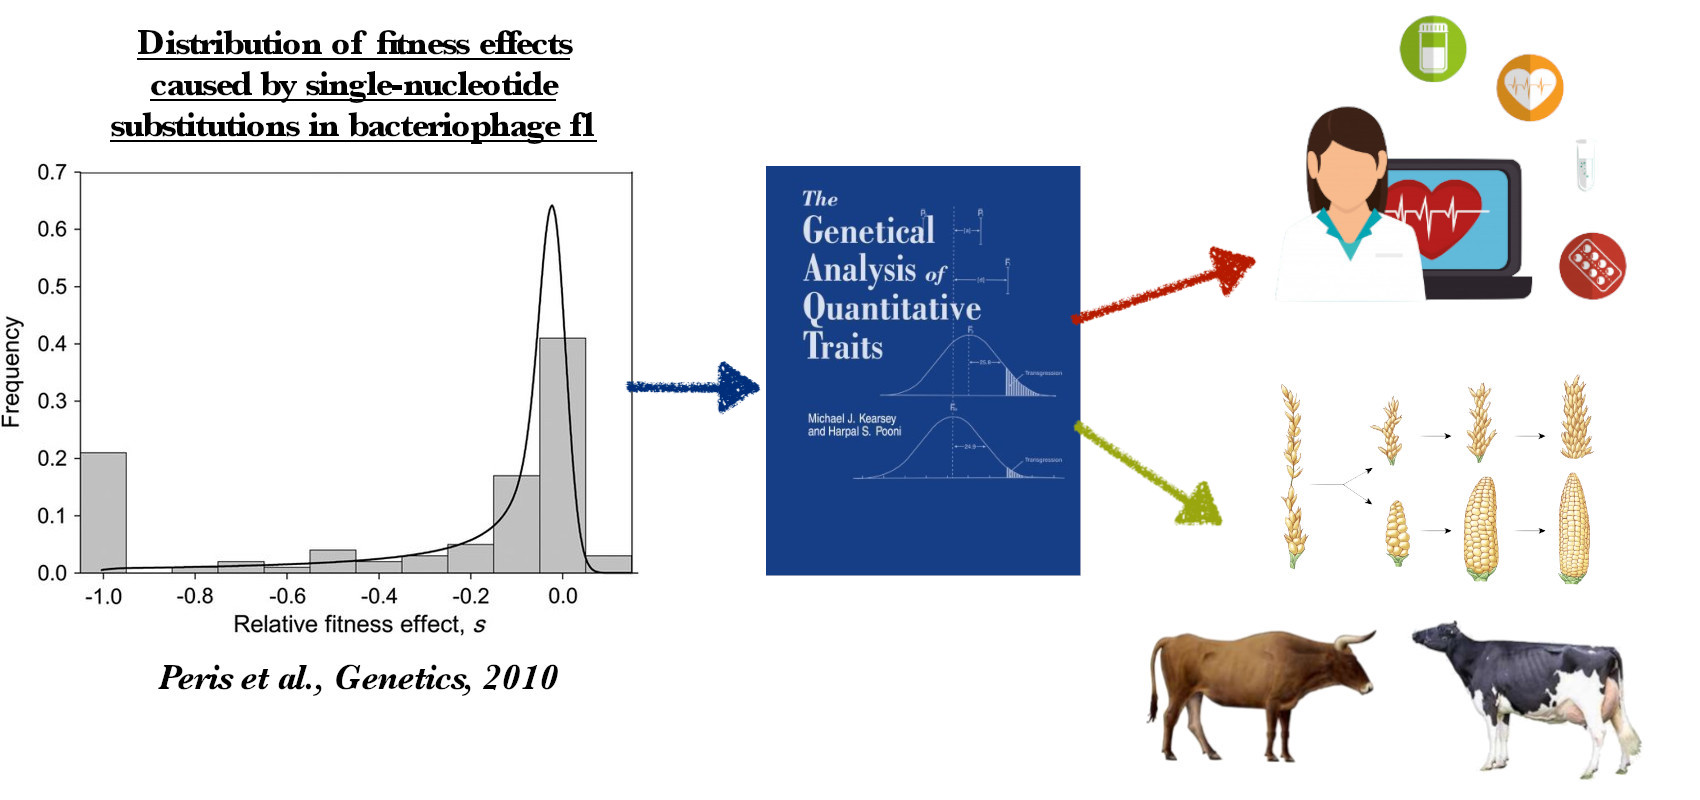
\includegraphics[scale=0.2]{img/DFE_phage_2010.jpg}
  \end{centering} 
\end{frame}

\begin{frame}
  \frametitle{Modèle}
  On pose
  \[
  \begin{array}{r l l}
    W_t &&\comment{fitness (taux de croissance) au temps $t$}\\
    s_i&=\frac{W_{t_{i-1}}-W_{t_i}}{W_{t_{i-1}}}&\comment{effet \emph{relatif} de la mutation $i$}\\
    N_t &&\comment{nombre de mutations avant le temps $t$}
  \end{array}
  \]

\vspace{0.5cm}%\pause

  \textbf{Énoncé du problème:} estimer la loi des $s_i$ (qui sont iid) sachant que l'on sait estimer la loi des $W_t$ et $N_t$ ($t\geqslant 0$), et sachant que \[\frac{W_t}{W_0}=\prod_{i=1}^{N_t}(1-s_i)\]
\end{frame}



\begin{frame}
  \frametitle{Plan}
  \tableofcontents
\end{frame}

\section{Expérience \& simulations}
\begin{frame}
  \sectionpage
\end{frame}

\begin{frame}
  \frametitle{Expérience: accumulation de mutations}
  \center\includegraphics[scale=0.3]{../Img/schema_microMA.png}
  \flushright{\emph{Robert et al.}, 2018}
  \end{frame}

\begin{frame}
  \frametitle{Expérience: accumulation de mutations}
  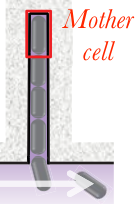
\includegraphics[scale=0.3]{../Img/Mother_cell.png}
  \includemedia[width=0.8\linewidth, height=0.4\linewidth,
  activate=pageopen, passcontext, transparent,
  addresource=../Video/microMA.mp4,
  flashvars={source=../Video/microMA.mp4}]{}{VPlayer.swf}
  \flushright{\emph{Robert et al.}, 2018}
  \end{frame}

%\begin{frame}
%  \frametitle{Expérience: visualisation de mutations}
%  \center\includegraphics[scale=0.5]{../Img/schema_MV.png}
%  \flushright{\emph{Robert et al.}}
%\end{frame}
%
%\begin{frame}
%  \frametitle{Expérience: visualisation de mutations}
%  \center\includemedia[width=\linewidth, height=0.4\linewidth,
%  activate=pageopen, passcontext, transparent,
%  addresource=../Video/MV.mp4,
%  flashvars={source=../Video/MV.mp4}]{}{VPlayer.swf}
%  \flushright{\emph{Robert et al.}}
%\end{frame}

\begin{frame}
\frametitle{Simulations: image}
\centering
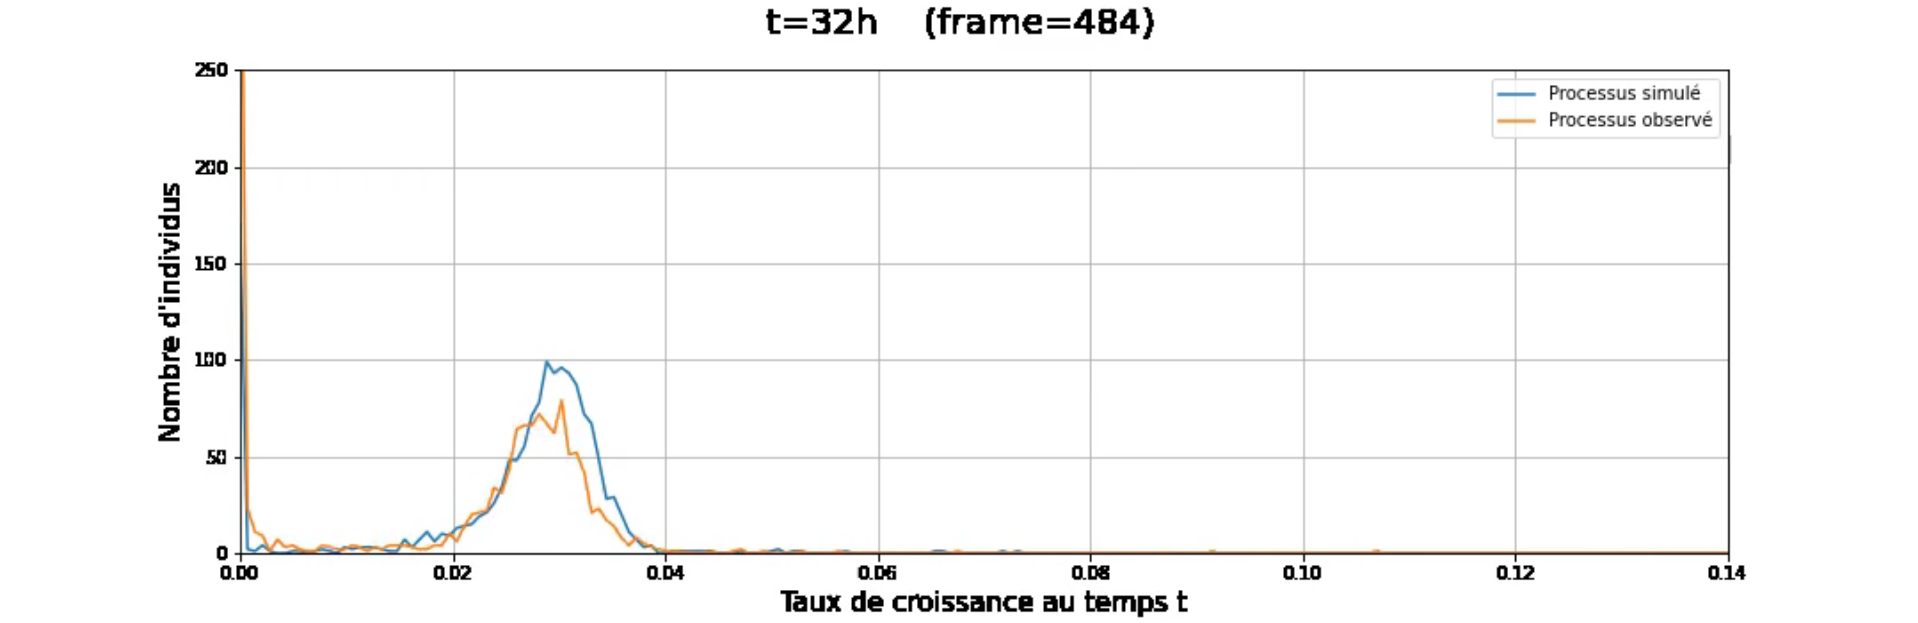
\includegraphics[scale=0.18]{img/proj_sshot_ani1.png}

\end{frame}

\begin{frame}
  \frametitle{Simulations}
  \center\includemedia[width=\linewidth, height=0.32\linewidth,
  activate=pageopen, passcontext, transparent,
  addresource=vid/GrowthRates_noisySimulations_VS_observations.mp4,
  flashvars={source=vid/GrowthRates_noisySimulations_VS_observations.mp4}]{}{VPlayer.swf}
\end{frame}


\section{Problème des moments}

\begin{frame}
  \sectionpage
\end{frame}

\subsection{Fonction caractéristique}

\begin{frame}
  \frametitle{Estimation des moments}

  \framesubtitle{Analyse de \emph{Robert et al.}, 2018}

  
\textbf{Moments} de la loi des effets des mutations;
 \[E_n(t):=\sum_{k=1}^n\binom{n}{k}(-1)^k\ln\pth{\Esp{W_t^k}}=\pth{\lambda\Esp{S^n}}t\]
 \pause
    \vspace{0.7cm}
 \begin{centering}
 
    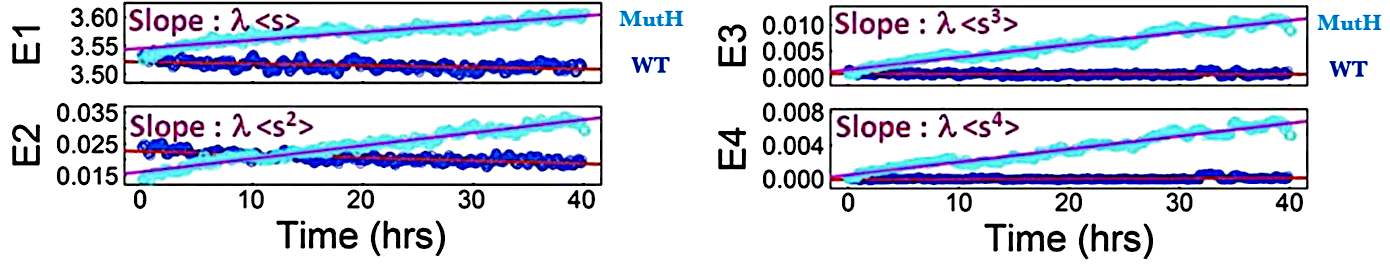
\includegraphics[scale=0.55]{img/Moments_estimation.png}
 \end{centering}
    \vspace{0.7cm}
 
$\to$ estimation facile des $\Esp{S^n}$.
\end{frame}


\begin{frame}
  \frametitle{Méthode par la fonction caractéristique}
  
  \begin{itemize}[label=$\bullet$]
  \item Moments $\to$ fonction caractéristique $\varphi_S$: 
    \[\varphi_S(\xi):=\Esp{e^{i\xi S}}=\sum_{k=0}^{+\infty}\frac{(i\xi)^k}{k!}\Esp{S^k}\]
    \pause
  \item Fonction caractéristique $\varphi_S$ $\to$ densité $f$ de la loi de $S$.
    \[f(x) = \frac1{2\pi} \int_{\mathbb R}\varphi_S(\xi)e^{-ix\xi}\de\xi\]
    \pause
  \item Avec les $N$ premiers moments estimés $m_k$:
    \begin{align*}
      \hat{\varphi}_S(\xi)=\sum_{k=0}^{N}\frac{(i\xi)^k}{k!}m_k
      \et\hat{f}(x)= \frac1{2\pi} \int_{\abs{\xi}\leqslant A}\hat\varphi_S(\xi)e^{-ix\xi}\de\xi
    \end{align*}
%    \pause
    \vspace{0.3cm}
    
  \item  \textbf{Espoirs:} $\varphi_S(\xi)\simeq \hat{\varphi}_S(\xi)$ donc $f(x)\simeq\hat{f}(x)$.
  \end{itemize}
  
\end{frame}


\subsection{Calculs d'erreurs}

\begin{frame}[allowframebreaks]
  \frametitle{Calculs d'erreurs}
  \prop{Pour tous paramètres $A>0$, $k\geqslant 2$, $N\geqslant 1$ on a : $\forall x\in\Er$
    \begin{align*}
      \abs{\hat{f}(x)-f(x)}&\leqslant\underbrace{\frac{\dabs{f^{(k)}}_1}{2\pi^2(k-1)A^{k-1}}}_{\text{erreur de régularisation}}\\
      &+\underbrace{\frac{A^{N+1}}{\pi(N+1)!}\Esp{S^N(e^{AS-1})}}_{\text{nb fini de moments}}+\underbrace{\frac{\dabs{\varepsilon(N)}_{\infty}(e^A-1)}{\pi}}_{\text{erreur sur les moments}}
    \end{align*}
    
    }
  %\pause
  \prop{Si:
    \begin{itemize}[label=$\bullet$]
    \item erreur sur les $\Esp{S^n}$ bornée par $\varepsilon$ (pour tout $n\in\En$);
    \item$\dabs{f^{(2)}}_1<+\infty$,
    \end{itemize}
    alors:
    \[\dabs{f-\hat{f}}_{\infty}=O\pth{\abs{\frac{1}{\ln^2(\varepsilon)}}}\comment{quand $\varepsilon\to 0$}\]
    }

\end{frame}

\section{EDP}

\begin{frame}
  \sectionpage
\end{frame}

\subsection{Nouveau point de vue}

\begin{frame}
  \frametitle{Un autre point de vue: une EDP}

  On a \[\ln W_t=\sum_{i=1}^{N_t}\ln(1-s_i)\]
  Soient:
\begin{itemize}[label=$\bullet$]
\item $u(t,\cdot)\in C^{\infty}(\Er)$: densité de $\mathcal{L}(\ln W_t)$;
\item $m(t)$: proportion de cellules mortes en $t$

$\to$ Loi de $\ln W_t$ :
\[\label{def_u} m(t)\delta_{-\infty}+u(t,\cdot)\]
\pause
\item $f(\cdot)\in C^{\infty}(\Er)$: densité de $\mathcal{L}(\ln(1-S))$;
\item $\mu$: proportion de mutations létales

$\to$ Loi de $\ln (1-S)$ :
\[\mu\delta_{-\infty}+f(\cdot)\]
%\pause
\item $\lambda$: taux de mutation
\end{itemize}

\end{frame}
\begin{frame}
  \frametitle{EDP et explication des termes}

Donc $(*)$:
\[\dr_tu(t,x)=\lambda\pth{{\red +}\int_{\Er}f(x-y)u(t,y)\de y{\blue -}\int_{\Er}f(y)u(t,x)\de y}-\lambda\mu u(t,x)\]

\vspace{0.5cm}

Traduction:%\pause
\begin{itemize}[label=$\bullet$]
\item $\dr_tu$: changement de densité de $\ln$-fitness entre $t$ et $t+\de t$;
\item $\int f(x-y)u(t,y)\de y$: arrivées sur la $\ln$-fitness x;
\item $-\int f(y)u(t,x)\de y$: départs de la $\ln$-fitness x;
\item $-\lambda\mu u(t,x)$: morts.
\end{itemize} 

\vspace{0.5cm}%\pause

Conservation de la masse : $$\int_{\Er} u(t,x)\de x=N(t)=e^{-\lambda\mu t}N(0)$$

\end{frame}


\begin{frame}
  \frametitle{Solution explicite}
%  La transformée de Fourier sur :
%  \[\dr_tu(t,x)=\lambda\pth{\int_{\Er}f(x-y)u(t,y)\de y-u(t,x)\int_{\Er}f(y)\de y}-\lambda\mu u(t,x)\]
%  donne
%  \[\dr_t\fr u_t(\xi)=\lambda \fr f(\xi)\fr u_t(\xi)-\lambda\fr u_t(\xi)\]
%  \pause
%  d'où:
\prop{
    Pour tout $x\in\mathbb{R}$:
    \[f(x)=\fr^{-1}\pth{\frac{\dr_t\pth{\fr u_t(\xi)}}{\lambda\fr u_t(\xi)}+1}\visible<2->{=\fr^{-1}\pth{\frac{a_{\xi}}{\lambda}+1}}\]%=\fr^{-1}\pth{\frac{1}{\lambda}\dr_t\ln\pth{\fr u_t(\xi)}+1}(x)\]
}

Terme de droite indépendant du temps \visible<2->{: $\dr_t(\fr u_t(\xi))=a_{\xi}\fr u_t(\xi)$.}

\pause
\vspace{0.5cm}

D'où:
\begin{align*}
  \fr u_t(\xi)&=e^{a_{\xi}t}\fr u_0(\xi)\\
  \ln\abs{\fr u_t(\xi)}&=\ln\abs{\fr u_0(\xi)}+t\times\Re(a_{\xi})\\
  \arg\pth{\fr u_t(\xi)}&=\arg{\fr u_0(\xi)}+t\times\Im(a_{\xi})
\end{align*}
\end{frame}

\subsection{Applications}


\begin{frame}
%[allowframebreaks]
  \frametitle{Vérification}
  
\begin{align*}
  \ln\abs{\fr u_t(\xi)}&=\ln\abs{\fr u_0(\xi)}+t\times\Re(a_{\xi})\\
  \arg\pth{\fr u_t(\xi)}&=\arg{\fr u_0(\xi)}+t\times\Im(a_{\xi})
\end{align*}
\pause

\vspace{0.3cm}
\begin{figure}
  
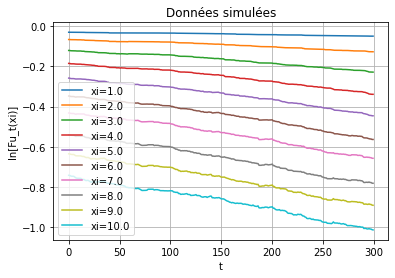
\includegraphics[scale=0.4]{img/proj_non_norm_sim}
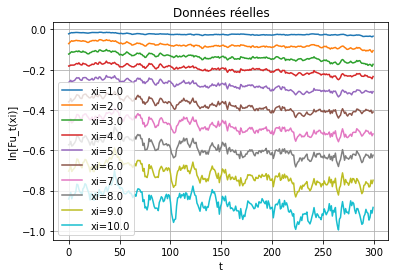
\includegraphics[scale=0.4]{img/proj_non_norm_rea}
  \caption{Graphes de $t\mapsto \ln\abs{\fr u_t(\xi)}$ pour données simulées et expérimentales.}
  
\end{figure}


\end{frame}

%
%\begin{frame}
%  \frametitle{Inférence des $a_{\xi}$}
%
%\begin{figure}[h]
%  \begin{center}
%    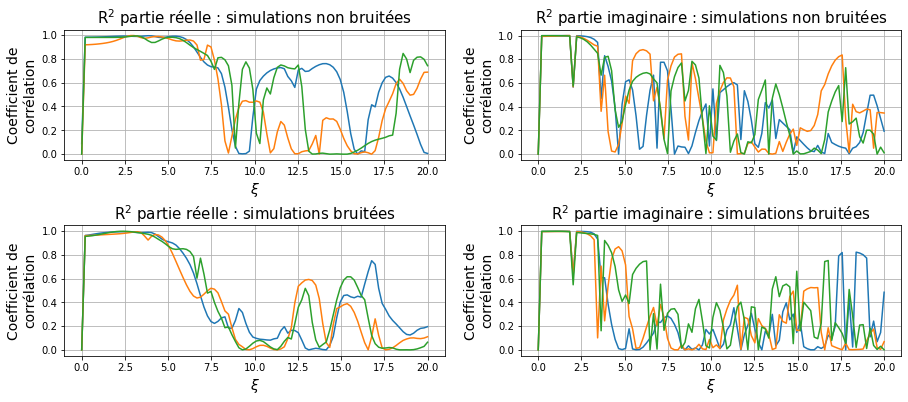
\includegraphics[width=0.9\linewidth]{../Img/DFE_R2.png}
%  \end{center}
%  \caption{\label{fig:DFE_R2}\textbf{Comparaison, selon $\xi$, des qualité d'ajustement d'un modèle affine} pour $t\mapsto \dr_t\fr u_t(\xi)$}
%\end{figure}
%
%%\vspace{0.5cm}
%
%\begin{itemize}[label=$\bullet$]
%\item fonctionne bien pour les petits $\xi$;
%\item fonctionne très mal pour les grands $\xi$ ($\to$ overfitting ?).
%\end{itemize}
%
%\end{frame}
%


\begin{frame}
  \frametitle{Mauvais résultats}
  
  \begin{figure}[h]
    \begin{center}
      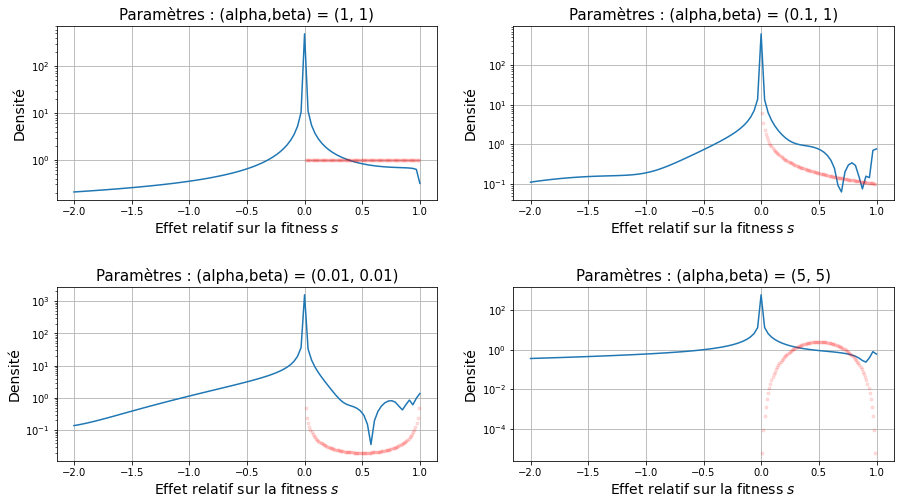
\includegraphics[width=0.9\linewidth]{../Img/DFE_inferred.png}
    \end{center}
    \caption{\label{fig:DFE}Comparaison entre les DFE inférées (en bleu) et les lois Beta choisies pour effectuer les simulations (en rouge). Utilisation de $f(x)=\fr^{-1}\pth{\frac{a_{\xi}}{\lambda}+1}$}
  \end{figure}


\end{frame}

%\begin{frame}[allowframebreaks]
%  \frametitle{Simulation avec grand nombre de canaux}
%  On enlève ?
%  
%  * droites magnifiques
%
%  * stabilité pour $\xi_{max}$ petit
%
%  * non-stabilité pour $\xi_{max}$ grand
%\end{frame}


\section*{Perspectives}

\begin{frame}
  \frametitle{Conclusion et perspectives}
  \begin{itemize}[label=$\bullet$]
    \item Problème inverse sévèrement mal posé;
    \vspace{3mm}
    \item 3 approches : Analyses naïves, Problème des moments, EDP \\
    $\to$ méthodes insuffisantes en pratique;
    \vspace{3mm}\pause
    \item Notebooks annotés : analyses reproductibles\\
    $\to$ en attente de données plus nombreuses ou moins bruitées;
    \vspace{3mm}\pause
    \item Améliorations :
    \begin{itemize}[label=$\star$]
    	\item Combinaison EDP + estimation des moments; 
	\item Similitudes avec les problèmes de fragmentation;          
	\item Propriétés de la DFE;
        \item Résultats théoriques sur l'erreur;
    \end{itemize}
    $\to$ simulations efficaces pour tester ces approches.
  \end{itemize}
\end{frame}



\begin{frame}
  \frametitle{Références}

  \begin{center}
    \Large{Merci pour votre attention !}
  \end{center}
  
\begin{thebibliography}{1}

\bibitem{rob}
  Robert et al.,
  \emph{Mutation dynamics and fitness effects followed in single cells}, Science 359, 1283–1286, 16 March 2018
\bibitem{mac}
  Trudy F. C. Mackay, Eric A. Stone, Julien F. Ayroles,
  \emph{The genetics of quantitative traits: challenges and prospects}, Nature Reviews Genetics, 565–577, 2009\bibitem{dou1}
  Doumic, Escobedo,
  \emph{Time asymptotics for a critical case in fragmentation and growth-fragmentation equations}, submitted 2015
\bibitem{dou2}
  Beal et al.,
  \emph{The Division of Amyloid Fibrils: Systematic Comparison of Fibril Fragmentation Stability by Linking Theory with Experiments}, iScience, 25 September 2020
\end{thebibliography}


\end{frame}





\end{document}
